%
% Permission is granted to copy, distribute and/or modify this
% document under the terms of the Creative Common by-nc-sa License
% version 3.0 (CC BY-NC-SA 3.0). A copy of the license can be found at
% http://creativecommons.org/licenses/by-nc-sa/3.0/legalcode.
%

%% Slides Class
\documentclass[10pt,a4paper]{beamer}


\usepackage[french]{babel}

%% Setting beamer style
\usepackage{UBdx}

%% Font packages
\usepackage{lmodern}
\usepackage[T1]{fontenc}
\usepackage[utf8]{inputenc}
% Highlight macros
\newcommand{\highlight}[1]{\textcolor{structure.fg}{\bfseries #1}}

\renewcommand{\cal}{\mathcal}
\newcommand{\setF}{\ensuremath{\mathbb{F}}\xspace}
%% Title, subtitle, authors, institute, date, ...
\title{Chiffrement de zones de stockage centralisées en environnement Linux (HPC)}

%\author{ZIRRI Yassine}
\author[ZIRRI Yassine]{ZIRRI Yassine\\[-.25em]
\texttt{\scriptsize <yaszirri@etu.u-bordeaux1.fr>}}
%\author[John Smit]{John Smith\\[-.25em]
%\texttt{\scriptsize <john.smith@etu.u-bordeaux.fr>}}
%\author[John Smith]{John Smith\\[-.25em]
%\texttt{\scriptsize <john.smith@etu.u-bordeaux.fr>}}
%\author[John Smih]{John Smith\\[-.25em]
%\texttt{\scriptsize <john.smith@etu.u-bordeaux.fr>}}

\institute[Master CSI, France]{Master CSI, Université de Bordeaux, France}

\date{\today}

%%%%%%%%%%%%%%%%%%%%%%%%%%[ Document ]%%%%%%%%%%%%%%%%%%%%%%%%%%
\begin{document}

\begin{frame}
  \vspace{3.5em}
  \titlepage

  \begin{center}
    
\includegraphics[scale=.2]{cc-by-nc-sa.pdf}
  \end{center}
\end{frame}

\begin{frame}
  \frametitle{Plan}
  \tableofcontents[subsectionstyle=hide]
\end{frame}

%%%%%%%%%%%%%%%%%%%%%%%%%%%%%%%%%%%%%%%%%%%%%%%%%%%%%%%%%%%%%%%%%%%%%%
\section{Gluster File System}

\begin{frame}
  \frametitle{GlusterFS}

\begin{itemize}
\item[•] GlusterFS est un système de fichiers libre distribué en parallèle.
\vfill
\item[•] Les serveurs sont déployés comme des << briques de stockage >>.\\
Chaque serveur exécutant un daemon glusterfsd qui exporte un système de fichier local comme << volume >>.
\vfill
\item[•] Le processus client glusterfs regroupe les volumes distants en un unique volume.\\
Le volume résultant est alors monté par un mécanisme FUSE.
\vfill
\item[•] La plupart des fonctionnalités sont implémentées comme "traducteurs" :\\
\begin{itemize}
\item[•] Duplication et Réplication par fichier.
\item[•] Partage de charge par fichier.
\item[•] Gestion des pannes.
\end{itemize}
\vfill
\end{itemize}

\end{frame}


\begin{frame}
  \frametitle{Lecture et Ecriture dans GlusterFS}

\begin{itemize}
\item[•] Mode distribué :\\
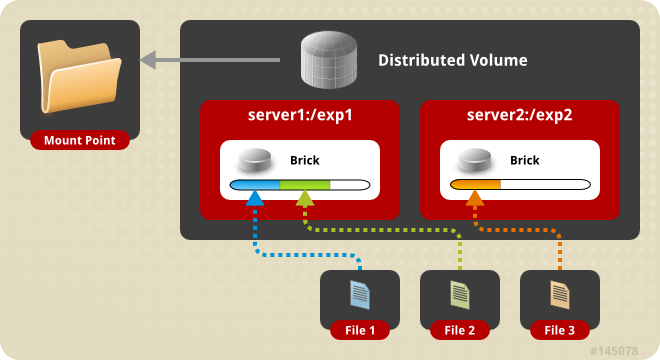
\includegraphics[width=10cm,height=2.5cm]{1.png}
\item[•] Mode répliqué :\\
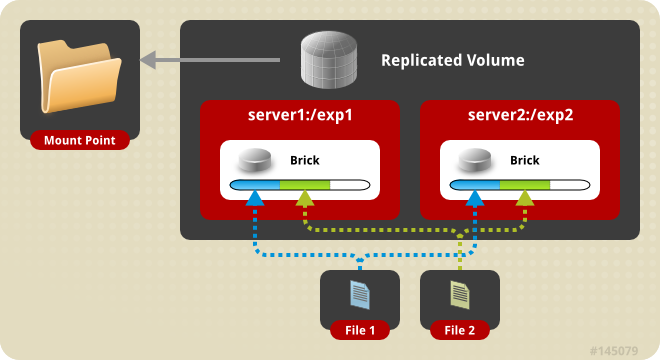
\includegraphics[width=10cm,height=2.5cm]{2.png}
\item[•] Mode striped :\\
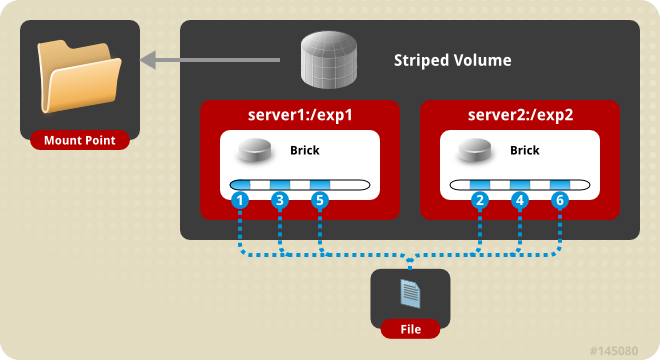
\includegraphics[width=10cm,height=2cm]{3.png}
\end{itemize}
\end{frame}

\begin{frame}
  \frametitle{Pourquoi choisir GlusterFS ?}

\begin{itemize}
\item[•] Il n'utilise pas de serveur central pour le stockage des metadata.\vfill
\item[•] Il peut grandir plus simplement que les autres DFS.\vfill
\item[•] GlusterFS server est conçu très simplement.\vfill
\item[•] Pour la confiance dans les nœuds (trust me).
\end{itemize}
\end{frame}

%%%%%%%%%%%%%%%%%%%%%%%%%%%%%%%%%%%%%%%%%%%%%%%%%%%%%%%%%%%%%%%%%%%%%%
\section{Encrypted File System}

\begin{frame}
  \frametitle{EncFS}

\begin{itemize}
\item[•] EncFS est un système de chiffrement qui fonctionne de façon simple sur tout système de fichiers grâce à FUSE.
\item[•] SECU : il utilise les algorithmes de la bibliothèques Libgcrypt de OpenSSL (AES, Blowfish,...).
\item[•] KERB : oui.
\item[•] GRAN : répertoire, fichier.
\item[•] ADMIN : facile.
\item[•] PRIX : open source (LGPL).
\item[•] Avantages : 
\begin{itemize}
\item[•] Installation facile et durable.
\item[•] Les performances semblent correctes.
\item[•] Fonctionnement possible sur différents types de système de fichier.
\end{itemize}
\item[•] Défauts  : 
\begin{itemize}
\item[•] Le dossier de stockage est visible => accès à quelques metadata (nombre de fichiers chiffrés, leur taille et droits d'accès).
\item[•] Absence de volume caché.
\end{itemize}
\end{itemize}

\end{frame}

%%%%%%%%%%%%%%%%%%%%%%%%%%%%%%%%%%%%%%%%%%%%%%%%%%%%%%%%%%%%%%%%%%%%%%
\section{VeraCrypt}

\begin{frame}
  \frametitle{VeraCrypt}
 \begin{itemize}
\item[•] VeraCrypt est un logiciel libre qui permet le cryptage des fichiers et partitions sous forme de conteneur global ou fichier unique.
\item[•] SECU : il utilise des algorithmes comme AES, Blowfish, Serpent...
\item[•] KERB : ...
\item[•] GRAN : disque, partition, répertoire et fichier.
\item[•] ADMIN : facile.
\item[•] PRIX : open source.
\item[•] Avantages : 
\begin{itemize}
\item[•] Installation facile et durable.
\item[•] Le logiciel et les fichiers sont compatibles multiplateformes.
\end{itemize}
\item[•] Défauts  : 
\begin{itemize}
\item[•] La robustesse de la protection est liée à la clef (minimum 15 caractères).
\item[•] le container est de taille fixe.
\end{itemize}
\end{itemize} 
  
\end{frame}

\end{document}
